\documentclass{article}
\usepackage[utf8]{inputenc}
\usepackage[T1]{fontenc}
\usepackage[english]{babel}
\usepackage{graphicx}
\usepackage{physics}
\usepackage{calrsfs}
\usepackage{mathalpha}
\usepackage{amssymb}
\usepackage{amsfonts}
\usepackage{amsmath}
\usepackage{fixltx2e}
\usepackage{enumitem}
\usepackage{float}
\usepackage[table]{xcolor}
\newcommand*\xor{\mathbin{\oplus}}
\usepackage{xcolor}
\usepackage{braket}
\usepackage{tikz}
\usepackage{hyperref}
\hypersetup{
  colorlinks=true,
  linkcolor=blue
}
\renewcommand{\labelitemi}{-}
\renewcommand{\labelitemii}{+}

\usepackage[dvipsnames]{xcolor}

\definecolor{myDarkGreen}{RGB}{0, 128, 0}

\title{Lesson 2021-06-01}
\begin{document}
\date{}
\maketitle
\section{Key Estabilishment, Distribution and Authentication in networks}
With the cryptographic mechanisms that we have learned so far, in particular symmetric and asymmetric encryption, digital signatures and message authentication
codes (MACs), one can relatively easily achieve the basic security services, i.e:
\begin{itemize}
    \item Confidentiality (with encryption algorithms)
    \item Integrity (with MACs or digital signatures)
    \item Message authentication (with MACs or digital signatures)
    \item Non repudiation (with digital signatures)
\end{itemize}
However, all cryptographic mechanisms that we have introduced so far assume
that keys are properly distributed between the parties involved, e.g., between Alice
and Bob. The task of key establishment is in practice one of the most important and
often also most difficult parts of a security system.\newline
Key estabilishment deals with estabilishing a shared secret between two or more parties, then it is going to be handled by proper protocols. We can derive that key estabilishment is \textbf{strongly related to identification}. For instance, you
may think of attacks by unauthorized users who join the key establishment protocol
with the aim of masquerading as either Alice or Bob with the goal of establishing a
secret key with the other party. To prevent such attacks, each party must be assured
of the identity of the other entity.\newline
We can define two main methods for key estabilishment, namely \textit{key transport} (in which one party generates and distributes the secret key) and \textit{key agreement} (in which parties jointly generate the key).
\newline Let's see an example of a classical key negotiation:
\newline Alice and Bob share a common password P. Using it they want to estabilish a secure key session.
\begin{figure} [H]
    \centering
    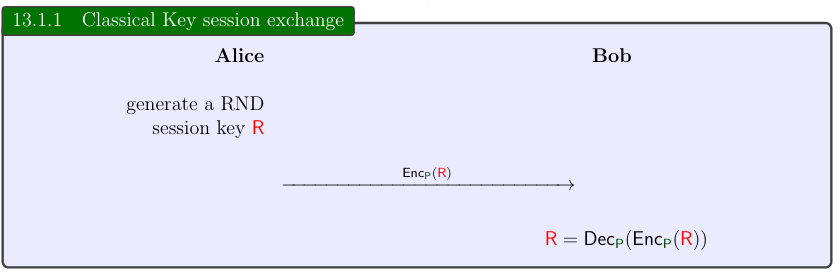
\includegraphics[scale=0.4]{classical_keyExch.png}
\end{figure}
\newline 
Now they share \textcolor{red}{R} and can use it as a session key. For example Bob can reply to Alice $Enc_R(Terminal type:)$.
\newline However this protocol happens to be insecure and has flaws. For example an eavesdropper could record messages and run a dictionary attack against the password P. Namely, he can try a candidate P' to decrypt $Enc_p(R)$. In this way he gets the result \textcolor{red}{R'} and uses it to decrypt $Enc_R$ looking for expected english words (redundancy), using for example a brute-force strategy.
\newline Another weakness of this protocol is that it's vulnerable to reply attacks (in which the attacker may use old messages). As a consequence there protocols must incorporate safeguards, i.e \textbf{random challenges}.
\subsection{Key freshness and KDF}
In many (but not all) security systems it is desirable to use cryptographic keys which
are only valid for a limited time, e.g., for one Internet connection. Such keys are
called \textit{session keys} or \textit{ephemeral keys}. Limiting the period in which a cryptographic
key is used has several advantages:
\begin{enumerate}
    \item Less damage if the key is exposed.
    \item An attacker has less ciphertext available that was generated under one key, which can make cryptographic attacks much more difficult
    \item An attacker is forced to recover several keys if he is interested in decrypting larger parts of plaintext.
\end{enumerate}
How can key updates be realized?
The first approach is to simply execute
the key establishment protocols shown before over and over again. However, there are always certain costs associated with key establishment, typically with respect to additional communication connections and computations.
The second approach to key update uses an already established joint secret key
to derive fresh session keys. The principal idea is to use a key derivation function
(KDF).
\begin{figure} [H]
    \centering
    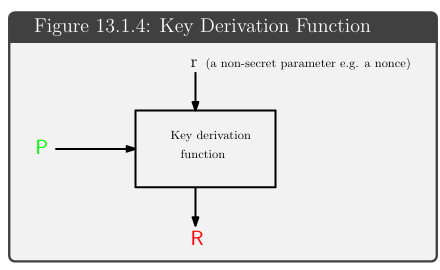
\includegraphics[scale=0.6]{kdf.png}
\end{figure}
An important characteristic of the key derivation function is that it should be a \textbf{one-way function}. The one-way property prevents an attacker from deducing $k_{AB}$
should any of the session keys become compromised, which in turn would allow the
attacker to compute all other session keys.
One possible way of realizing the key derivation function is that one party sends
a nonce, i.e., a numerical value that is used only once, to the other party. Both users
encrypt the nonce using the shared secret key $k_{AB}$ by means of a symmetric cipher
such as AES. The corresponding protocol is shown below
\begin{figure} [H]
    \centering
    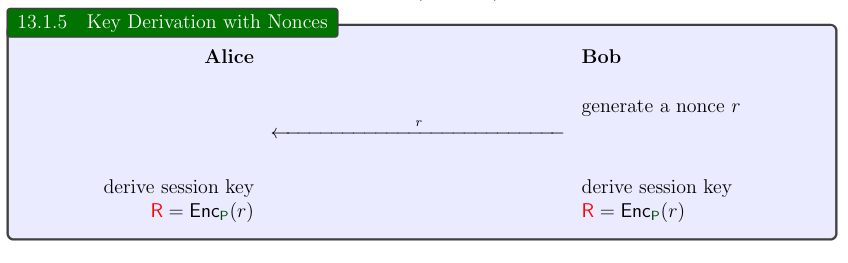
\includegraphics[scale=0.4]{kd_nonce.png}
\end{figure}
An alternative to encrypting the nonce is hashing it together with $k_{AB}$. One way of achieving this is that both parties perform a HMAC computation with the nonce serving as the message:
\begin{equation*}
    k_{ses} = HMAC_{k_{AB}}(r)
\end{equation*}
Rather than sending a nonce, Alice and Bob can also simply encrypt a counter $cnt$ periodically, where the ciphertext again forms the session key:
\begin{equation*}
    k_{ses} = e_{k_{AB}}(cnt)
\end{equation*}
or compute the HMAC of the counter, i.e:
\begin{equation*}
    k_{ses} = HMAC_{k_{AB}}(cnt)
\end{equation*}
Using a counter can save Alice and Bob one communication session because, unlike the case of the nonce-based key derivation, no value needs to be transmitted. However, this holds only if both parties know ecactly when the next key derivation needs to take place. Otherwise, a counter synchronization message might be required.
\subsection{Encrypted Key Exchange (EKE)}
This protocol is a combination of symmetric and asymmetric cryptography. It provides security and authentication on computer
networks, using both symmetric and public-key cryptography in a novel way:
A shared secret key is used to encrypt a randomly generated public key.
\begin{figure} [H]
    \centering
    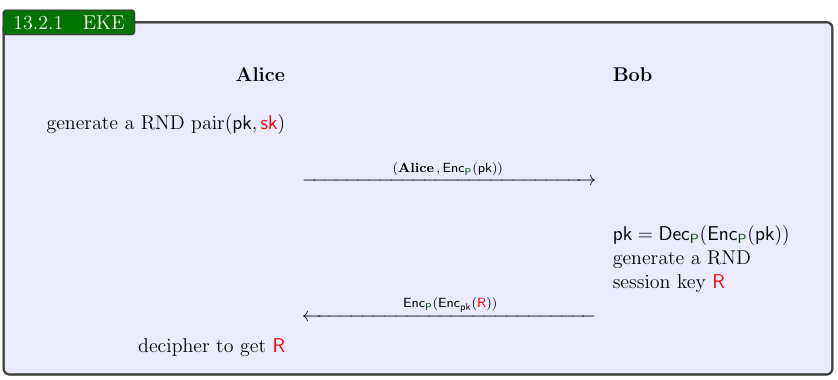
\includegraphics[scale=0.4]{eke.png}
\end{figure}
Let's explain the basic EKE protocol:

Alice and Bob (two users, a user and the host, or whoever) share a common
password, P. Using this protocol, they can authenticate each other and generate
a common session key, \textcolor{red}{R}.
\begin{enumerate}
    \item Alice generates a random public-key/private-key key pair. She
encrypts the public key, pk (in order to avoid dictionary attack, i.e in this way we solve the weakness of classical key exchange protocol), using a symmetric algorithm and P as the
key: $Enc_P(pk)$. She sends Bob $(Alice, Enc_P(pk))$. In this case a dictionary attack against the public key is computationally unfeasible (we are not dealing with english words).
    \item Bob knows P. He decrypts the message to obtain pk. Then, he
generates a random session key, \textcolor{red}{R}, and encrypts it with the public key
he received from Alice and P as the key. He sends Alice $Enc_P(Enc_{pk}(R))$
    \item Alice decrypts the message to obtain \textcolor{red}{R}. She generates a random string $R_A$ and encrypts it using \textcolor{red}{R}. Then she sends to Bob $Enc_{\textcolor{red}{R}}(R_A)$. At this step, both Alice and Bob know pk  and  \textcolor{red}{R}.  \textcolor{red}{R} is the session key and can
be used to encrypt all other messages between Alice and Bob. Oscar, sitting
between Alice and Bob, only knows $Enc_P(pk)$, $Enc_P(Enc_{pk}( \textcolor{red}{R})$, and some messages
encrypted with  \textcolor{red}{R}. In other protocols, Oscar could make guesses at P (people
choose bad passwords all the time, and if Oscar is clever he can make some
good guesses) and then test his guesses. In this protocol, Oscar cannot test his guess without cracking the public-key algorithm as well. And if both pk and  \textcolor{red}{R} are chosen randomly, this can be an insurmountable problem.
\item Bob decrypts the message to obtain $R_A$ . He generates another
random string, $R_B$ , encrypts both strings with \textcolor{red}{R}, and sends Alice the
result $Enc_{\textcolor{red}{R}}(R_A, R_B)$
\item Alice decrypts the message to obtain $R_A$ and $R_B$ . Assuming the $R_A$
she received from Bob is the same as the one she sent to Bob in step (3),
she encrypts $R_B$ with \textcolor{red}{R} and sends to Bob $Enc_{\textcolor{red}{R}}(R_B)$
\item Bob decrypts the message to obtain $R_B$ . Assuming the $R_B$ he
received from Alice is the same one he sent to Alice in step (4), the protocol is complete. Both parties now communicate using \textcolor{red}{R} as the
session key.
\end{enumerate}
The challenge-response portion of the protocol, steps (3) through (6), provides
validation. Steps (3) through (5) prove to Alice that Bob knows \textcolor{red}{R}; steps (4)
through (6) prove to Bob that Alice knows \textcolor{red}{R}.
\begin{figure} [H]
    \centering
    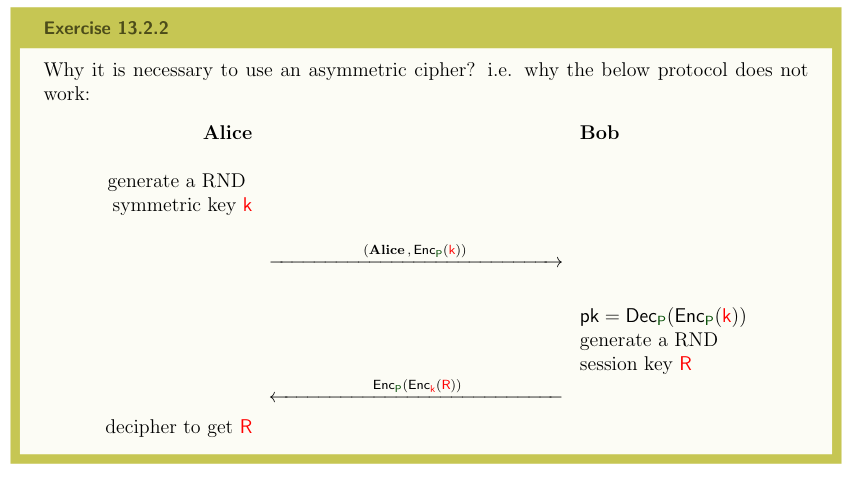
\includegraphics[scale=0.4]{ex13.2.2.png}
\end{figure}
\textcolor{red}{Solution:}
\newline
Basically we use asymmetric cipher in order to avoid dictionary attack. 
\newline Assuming that the attacker knows the cipher, let's explain the loop in which the dictionary attack happens.
Oscar (the attacker) picks a candidate secret P' from his dictionary file and uses it to obtain a candidate for $Enc_k(\textcolor{red}{R})$:
\begin{equation*}
    Dec_{P'}(Enc_P(Enc_k(\textcolor{red}{R})))
\end{equation*}
After that, having kept $Enc_P(k))$ from the insecure channel, Oscar can generate a candidate k':
\begin{equation*}
    Dec_{P'}(Enc_P(k)) = k'
\end{equation*}
At the end Oscar generates a candidate $\textcolor{red}{R'} = Dec_{k'}(Enc_k(\textcolor{red}{R}))$ that can be used to decrypt the traffic (in english) between Alice and Bob, because the cipher is symmetric, i.e we have just one key for both the parties.
\subsubsection{EKE using RSA and Partition Attacks}
Encryptions using a password P must leak no information. This is often quite difficult, simply because of the numerical properties of the cryptosystems used. For example, public keys in RSA are always odd. Knowing this fact, if no special precautions are taken, an attacker could rule out half of the candidate values $P'$ if $P'^{-1}(P(e))$ (where e belongs to the pair of large natural numbers $(e, n)$ used to generate the public key $E_A$ in RSA) were an even number. At first blush, this is an important reduction in the key space.
\newline Recall that each session will use a different public key,  independent of all others previously used.  Thus,trial  decryptions  resulting  in  illegal  values  of $e′$ will exclude different values of $P′$ each time.  Put in another way,  each session will partition the remaining candidate  key  space  into  two  approximately-equal  halves.The decrease in the keyspace is logarithmic.
\newline We  call  this  attack  a \textbf{partition attack}. For some cryptosystems, one may choose to accept a minimal partition.  Consider a situation where one must  encrypt,  with $P$ ,  integers  modulo  some  known prime $p$.  Clearly, if $n$ bits are needed to encode $p$, trial decryptions yielding values in the range $[p,2^{n−1}$ can be  used  to  partition  the  password  space.   However,if $p$ is  very  close  to  $2^n$ ,  perhaps  even  $2^{n−1}$,  very few candidates are excluded.  Conversely, values of $p$ near   $2^{n−1}$ are  quite  bad.   For  any  value  of $p$,  it  is obviously possible to calculate how many interceptions are necessary to analyze any given size password space.Another area of possible exposure comes from trying  to  encrypt  a  given  number  with  a  cryptosystem that demands a larger block size.  The straightforward way  to  do  this  —  inserting  high-order  zero  bits  — poses an obvious risk.  Instead,  those bits should be filled with random data.
\subsection{Validation of keys}
Once Alice and Bob have the session key \textcolor{red}{R}, there's the validation key problem. Let's see a standard technique for validating cryptographical keys:
\begin{figure} [H]
    \centering
    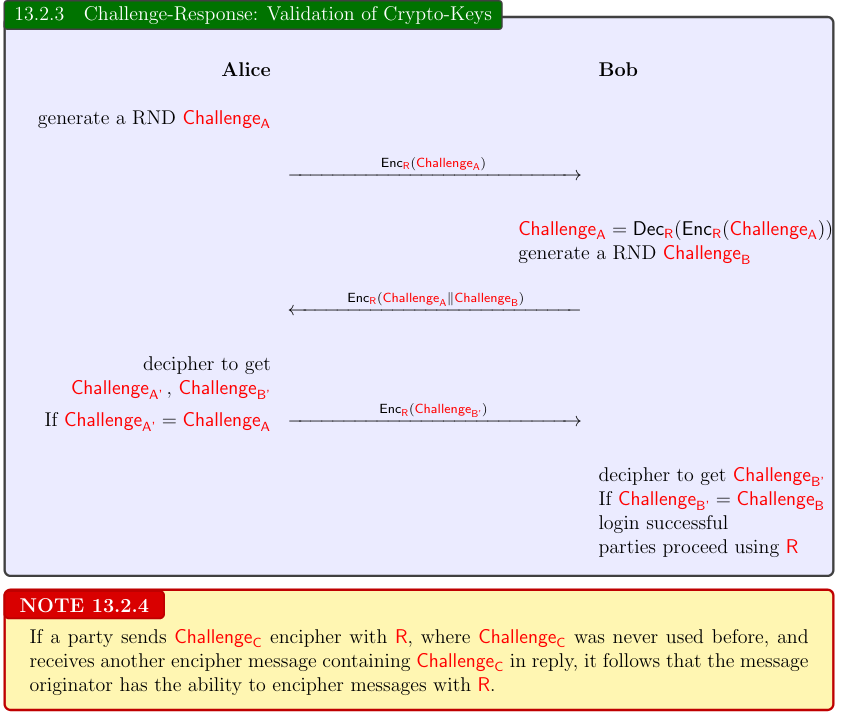
\includegraphics[scale=0.4]{challenge.png}
\end{figure}
As we can see in the picture above:
\begin{enumerate}
\item Alice generates a random $Challenge_A$. Recall: In computer security, challenge–response authentication is a family of protocols in which one party presents a question ("challenge") and another party must provide a valid answer ("response") to be authenticated. In our case we're trying to "authenticate" the session key. 
\item Alice encrypts her challenge with the session key and sends it to Bob
\item Bob recovers the $Challenge_A$ by decrpting it: 
\begin{equation*}
    Challenge_A = Dec_{\textcolor{red}{R}}(End_{\textcolor{red}{R}}(Challenge_A))
\end{equation*}
\item Bob generates his random challenge $Challenge_B$, then he concatenates it to $Challenge_A$ and sends it to A (obviously encrypted with \textcolor{red}{R})
\item Alice verifies her challenge by decrypting what he received from Bob. if $Challenge_{A'} = Challenge_A$, then she (encrypts with \textcolor{red}{R}) and sends $Challenge_{B'}$ to Bob
\item Bob verifies his challenge in the same way
\end{enumerate}
Now Alice and Bob can communicate using their session key \textcolor{red}{R}.
\subsection{Key Exchange Key (KEK)}
Suppose that a cryptanalyst has recovered some session key \textcolor{red}{R} (e.g.  by a trojan or by using the record of an old session protected by the EKE protocol).  Then he can attack the password $P$ e.g.  perform a dictionary and off-line attack.  Indeed, for $P’$ in the dictionary the attacker computes
\begin{equation*}
    pk' := Dec_{P'}(Enc_P(pk))
\end{equation*}
and checks if
\begin{equation*}
    Enc_P(Enc_{pk}(\textcolor{red}{R})) = Enc_{P'}(Enc_{pk'}(\textcolor{red}{R}))
\end{equation*}
To prevent this a true session key \textcolor{red}{S} can be obtained with a little variation of the Challenge-Response portion of the protocol seen before.  The \textcolor{red}{R} is now called a key exchange key (KEK).
A Key Encryption Key or KEK is simply a key that is solely used to encrypt keys. The keys that are encrypted are usually keys that have a specific meaning such as domain specific keys. It could also be that the encrypted keys have shorter life time such a as session keys.
\begin{figure} [H]
    \centering
    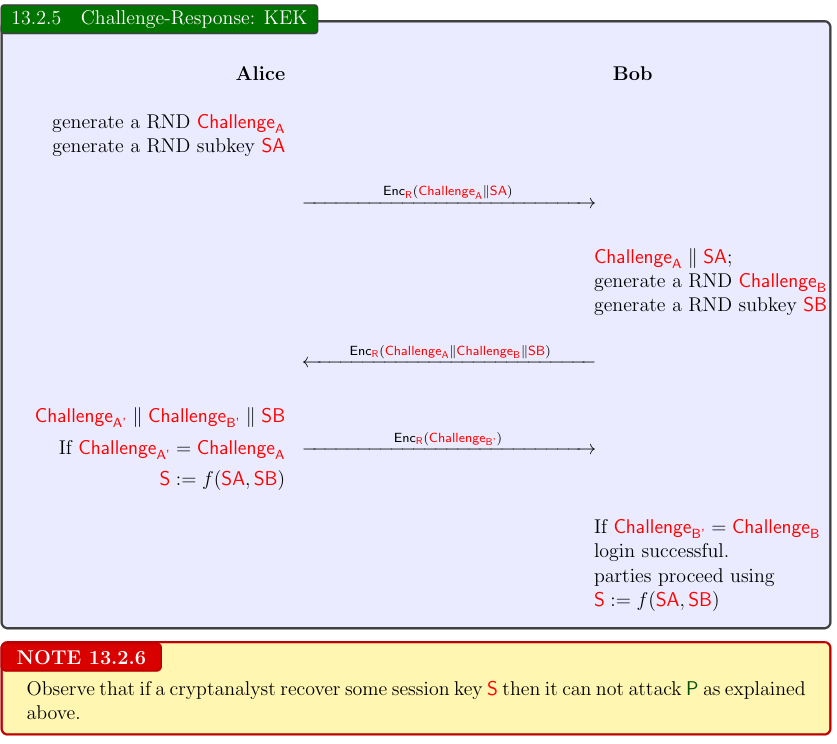
\includegraphics[scale=0.4]{kek.png}
\end{figure}
\subsection{Key Distribution Center (KDC)}
A KDC is a server that is fully trusted by all users and that shares a secret key $\textcolor{red}{k_U}$ with each user. $\textcolor{red}{k_U}$ is called Key Encryption Key (KEK)).
THe idea is to have a central \textbf{trusted} authority that shares one key with every user.
Let's explain how does it work:
\newline A necessary prerequisite is that each user shares a unique secret key $\textcolor{red}{k_U}$ KEK  with the key distribution center which predistributed through a secure channel. Let’s
look what happens if one party requests a secure session from the KDC, e.g., Alice
wants to communicate with Bob. The interesting part of this approach is that the
KDC encrypts the session key that will eventually be used by Alice and Bob. In
a basic protocol, the KDC generates two messages, y A and y B , for Alice and Bob, as we can see in the figure below
\begin{figure} [H]
    \centering
    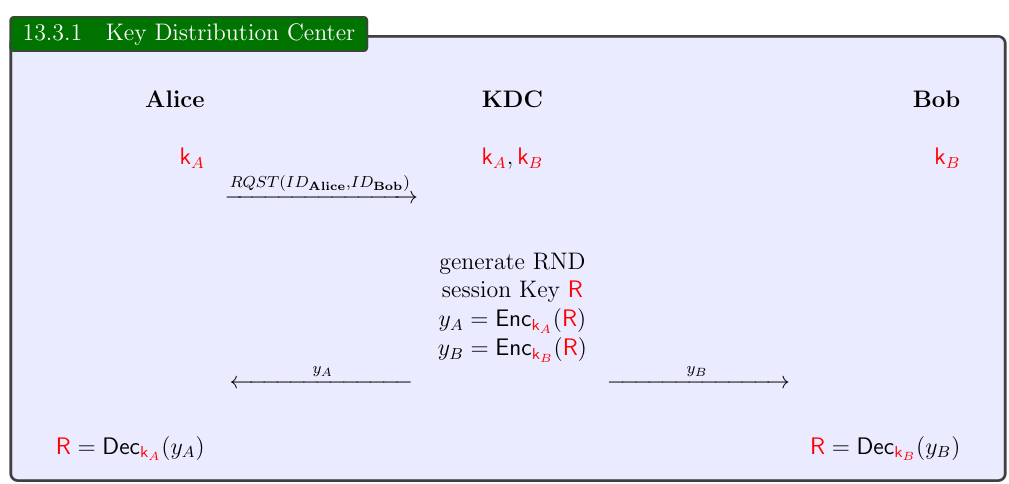
\includegraphics[scale=0.35]{kdc.png}
\end{figure}
Alice receives the session key encrypted with both KEKs, $k_A$ and $k_B$ . She is able
to compute the session key \textcolor{red}{R} from $y_A$ and can use it subsequently to encrypt the
actual message she wants to send to Bob, i.e $y = Enc_{\textcolor{red}{R}}(x)$. The interesting part of the protocol is that
Bob receives both the encrypted message $y$ as well as $y_B$ . He needs to decrypt the
latter one in order to recover the session key which is needed for computing x.
Both of the KDC-based protocols have the advantage that there are only n long-
term symmetric key pairs in the system. The n long-term KEKS only
need to be stored by the KDC, while each user only stores his or her own KEK. Most importantly, if a new user Noah joins the network, a secure channel only needs to
be established once between the KDC and Noah to distribute the KEK $k_N$.
\subsubsection{KDC Security}
Even if the above protocol protect against passive attacks it is really weak to active attacks:
\begin{enumerate}
    \item \textbf{Replay Attack}:This attack makes
use of the fact that neither Alice nor Bob know whether the encrypted session key
they receive is actually a new one. If an old one is reused, key freshness is violated.
This can be a particularly serious issue if an old session key has become compromised. This could happen if an old key is leaked, e.g., through a hacker, or if the
encryption algorithm used with an old key has become insecure due to cryptanalytical advances.
If Oscar gets hold of a previous session key, he can impersonate the KDC and
resend old messages $y_A$ and $y_B$ to Alice and Bob. Since Oscar knows the session
key, he can decipher the plaintext that will be encrypted by Alice or Bob.
    \item \textbf{Key Confirmation Attack}: Another weakness of the above protocol is that Alice
is not assured that the key material she receives from the KDC is actually for a
session between her and Bob. This attack assumes that Oscar is also a legitimate
(but malicious) user. By changing the session-request message Oscar can trick the
KDC and Alice to set up session between him and Alice as opposed to between
Alice and Bob. Here is the attack ($k_{ses}$ is the session key):
\begin{figure} [H]
    \centering
    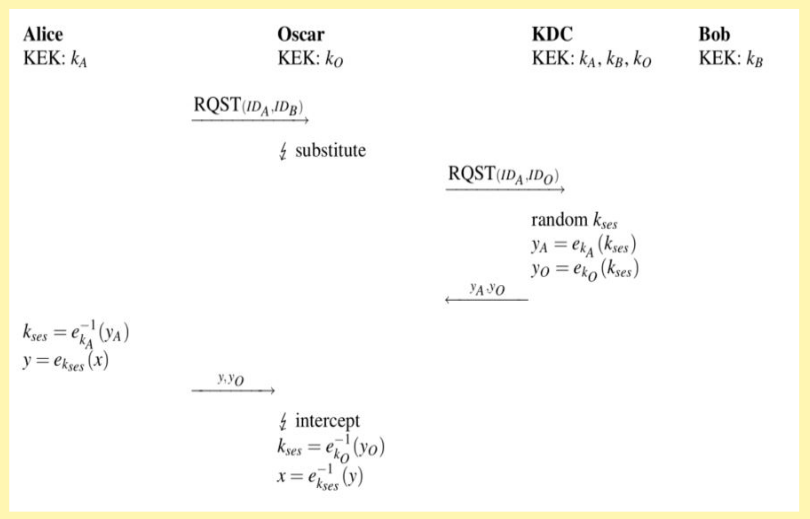
\includegraphics[scale=0.4]{key_confirm_attack.png}
\end{figure}
The gist of the attack is that the KDC believes Alice requests a key for a session
between Alice and Oscar, whereas she really wants to communicate with Bob. Alice
assumes that the encrypted key “$y_O$ ” is “$y_B$ ”, i.e., the session key encrypted under
Bob’s KEK $k_B$ . (Note that if the KDC puts a header ID O in front of y O which associates it with Oscar, Oscar might simply change the header to ID B .) In other words,
Alice has no way of knowing that the KDC prepared a session with her and Oscar;
instead she still thinks she is setting up a session with Bob. Alice continues with the
protocol and encrypts her actual message as y. If Oscar intercepts y, he can decrypt
it.
The underlying problem for this attack is that there is no key confirmation. If key
confirmation were given, Alice would be assured that Bob and no other user knows
the session key.
\end{enumerate}
\subsubsection{Kerberos}
A more advanced protocol that protects against both replay and key confirmation
attacks is Kerberos. It is, in fact, more than a mere key distribution protocol; its
main purpose is to provide user authentication in computer networks. Kerberos is also based on a KDC, which is named the “authentication sever” in Kerberos terminology. Let’s
first look at a simplified version of the protocol.
\begin{figure} [H]
    \centering
    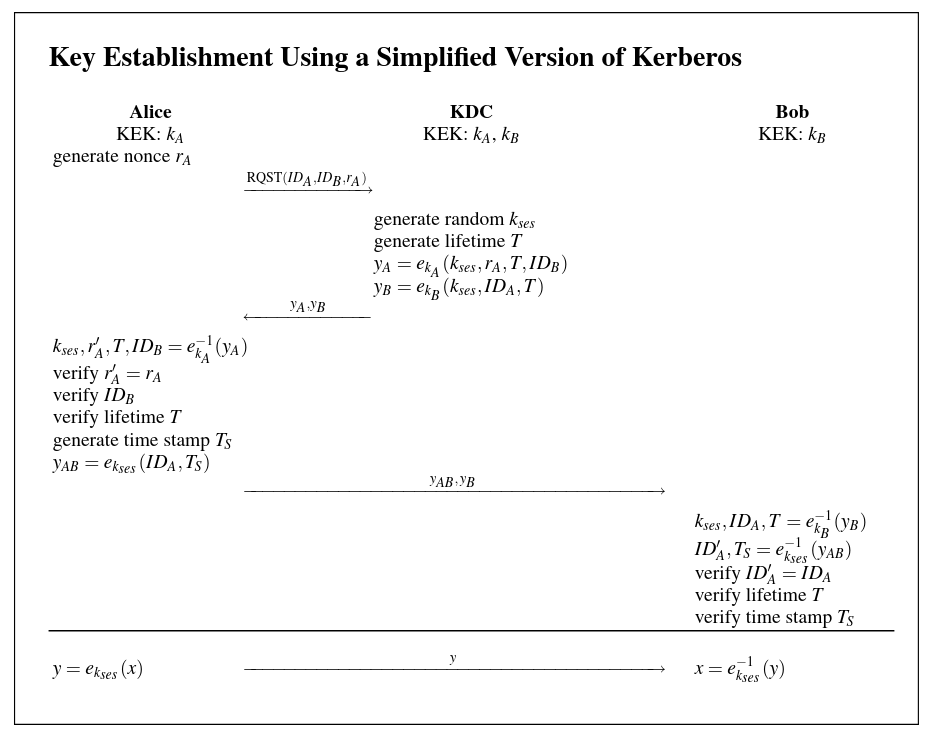
\includegraphics[scale=0.4]{kerberos.png}
\end{figure}
Kerberos assures the timeliness of the protocol through two measures. First, the
KDC specifies a lifetime T for the session key. The lifetime is encrypted with both
session keys, i.e., it is included in $y_A$ and $y_B$ . Hence, both Alice and Bob are aware
of the period during which they can use the session key. Second, Alice uses a time
stamp $T_S$ , through which Bob can be assured that Alice’s messages are recent and
are not the result of a replay attack. For this, Alice’s and Bob’s system clocks must
be synchronized, but not with a very high accuracy. Typical values are in the range
of a few minutes. The usage of the lifetime parameter T and the time stamp $T_S$
prevent replay attacks by Oscar.
Equally important is that Kerberos provides key confirmation and user authenti-
cation. In the beginning, Alice sends a random nonce $r_A$ to the KDC. This can be
considered as a challenge because she challenges the KDC to encrypt it with their
joint KEK $k_A$ . If the returned challenge $r_{A'}$ matches the sent one, Alice is assured that
the message $y_A$ was actually sent by the KDC. This method to authenticate users is
known as challenge-response protocol and is widely used, e.g., for authentication of
smart cards.
Through the inclusion of Bob’s identity $ID_B$ in $y_A$ Alice is assured that the session
key is actually meant for a session between herself and Bob. With the inclusion of
Alice’s identity $ID_A$ in both $y_B$ and $y_{AB}$ , Bob can verify that (i) the KDC included
a session key for a connection between him and Alice and (ii) that he is currently
actually talking to Alice.
\newline
Even though Kerberos provides strong assurance that the correct keys are being
used and that users are authenticated, there are still drawbacks to the protocols discussed so far. We now describe remaining general problems that exist for KDC-based schemes.
\begin{itemize}
    \item \textbf{Communication requirements } One problem in practice is that the KDC needs to
be contacted if a new secure session is to be initiated between any two parties in the
network. Even though this is a performance rather than a security problem, it can be
a serious hindrance in a system with very many users. In Kerberos, one can alleviate
this potential problem by increasing the lifetime T of the key. In practice, Kerberos
can run with tens of thousands of users. However, it would be a problem to scale
such an approach to “all” Internet users.
\item \textbf{Secure channel during initialization}  As discussed earlier, all KDC-based protocols require a secure channel at the time a new user joins the network for transmit-
ting that user’s key encryption key.
\item \textbf{Single point of failure}  All KDC-based protocols, including Kerberos, have the
security drawback that they have a single point of failure, namely the database that
contains the key encryption keys, the KEKs. If the KDC becomes compromised,
all KEKs in the entire system become invalid and have to be re-established using
secure channels between the KDC and each user.
\item \textbf{No perfect forward secrecy}  If any of the KEKs becomes compromised, e.g.,
through a hacker or Trojan software running on a user’s computer, the consequences
are serious. First, all future communication can be decrypted by the attacker who
eavesdrops. For instance, if Oscar got a hold of Alice’s KEK $k_A$ , he can recover the
session key from all messages $y_A$ that the KDC sends out. Even more dramatic
is the fact that Oscar can also decrypt past communications if he stored old
messages $y_A$ and y. Even if Alice immediately realizes that her KEK has been compromised and she stops using it right away, there is nothing she can do to prevent
Oscar from decrypting her past communication.
Therefore, a protocol has perfect forward secrecy (PFS) if the compromise of long-term keys does notallow an attacker to obtain past session keys.
\end{itemize}
\newline\newline \textcolor{red}{Exercise 13.3.5}: Convince yourself that protocol EKE has PFS. Keep in mind that the long-term key is P.
\newline \textcolor{red}{Solution}:
Perfect forward secrecy (PFS for short) refers to the property of key-exchange protocols (Key Exchange) by which the exposure of long-term keying material, used in the protocol to authenticate and negotiate session keys, does not compromise the secrecy of session keys established before the exposure.
In the case of authenticated key exchange protocols, where security is to be provided against active attackers, PFS means that the attacker cannot compute past session keys exchanged between honest parties even if the attacker actively interfered in the session creation.
Let's recall the EKE protocol:
\begin{figure} [H]
    \centering
    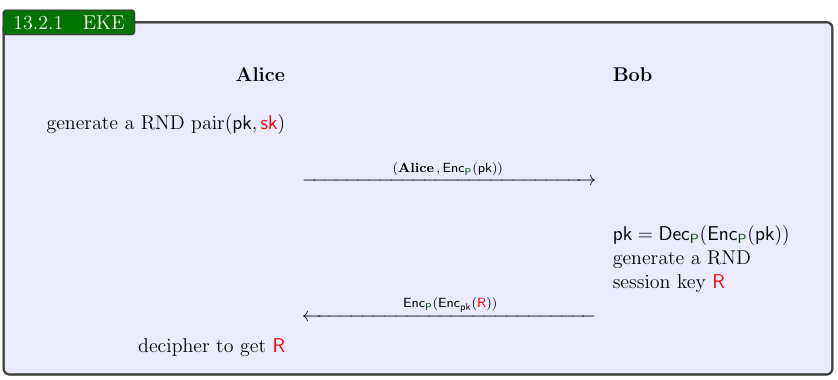
\includegraphics[scale=0.3]{eke.png}
\end{figure}
Basically this protocol has PFS because it exploits asymmetric cryptography.
In principle, any public key encryption scheme can be used to build a key exchange with PFS by using the encryption scheme with ephemeral public and private keys (such as Diffie-Hellman). 

\subsubsection{Wide-Mouth Frog protocol}
The Wide-Mouth Frog protocol is probably the simplest symmetric
key-management protocol that uses a trusted server. Both Alice and Bob share
a secret key with Trent. The keys are just used for key distribution and not to
encrypt any actual messages between users. Just by using two messages, Alice
transfers a session key to Bob:
\begin{figure} [H]
    \centering
    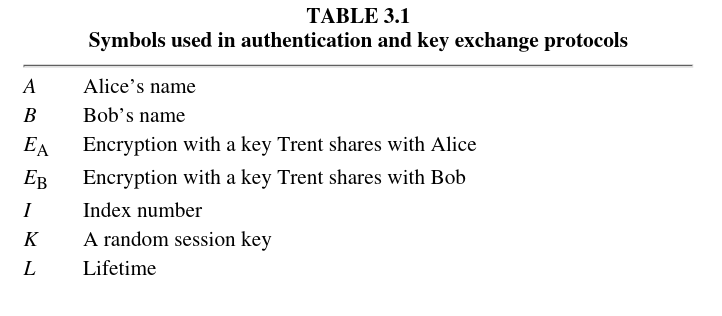
\includegraphics[scale=0.4]{table3.1.png}
    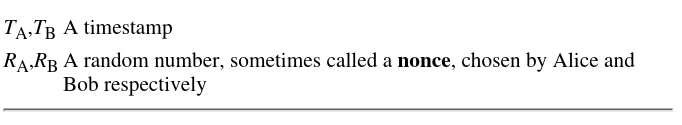
\includegraphics[scale=0.4]{table3.1.2.png}
\end{figure}
\begin{enumerate}
    \item Alice concatenates a timestamp, Bob’s name, and a random session
key and encrypts the whole message with the key she shares with Trent.
She sends this to Trent, along with her name.
\begin{equation*}
    A, E_A(T_A, B, K)
\end{equation*}
\item Trent decrypts the message from Alice. Then he concatenates a new
timestamp, Alice’s name, and the random session key; he encrypts the
whole message with the key he shares with Bob. Trent sends to Bob:
\begin{equation*}
    E_B(T_B, A, K)
\end{equation*}
\end{enumerate}
The biggest assumption made in this protocol is that Alice is competent
enough to generate good session keys. Remember that random numbers aren’t
easy to generate; it might be more than Alice can be trusted to do properly.
\subsubsection{Needham-Schroeder protocol}
The Needham–Schroeder protocol is one of the two key transport protocols intended for use over an insecure network, both proposed by Roger Needham and Michael Schroeder. These are:
\begin{enumerate}
    \item The Needham–Schroeder Symmetric Key Protocol, based on a symmetric encryption algorithm. It forms the basis for the Kerberos protocol. This protocol aims to establish a session key between two parties on a network, typically to protect further communication.
    \item     The Needham–Schroeder Public-Key Protocol, based on public-key cryptography. This protocol is intended to provide mutual authentication between two parties communicating on a network, but in its proposed form is insecure.
\end{enumerate}
\begin{figure} [H]
    \centering
    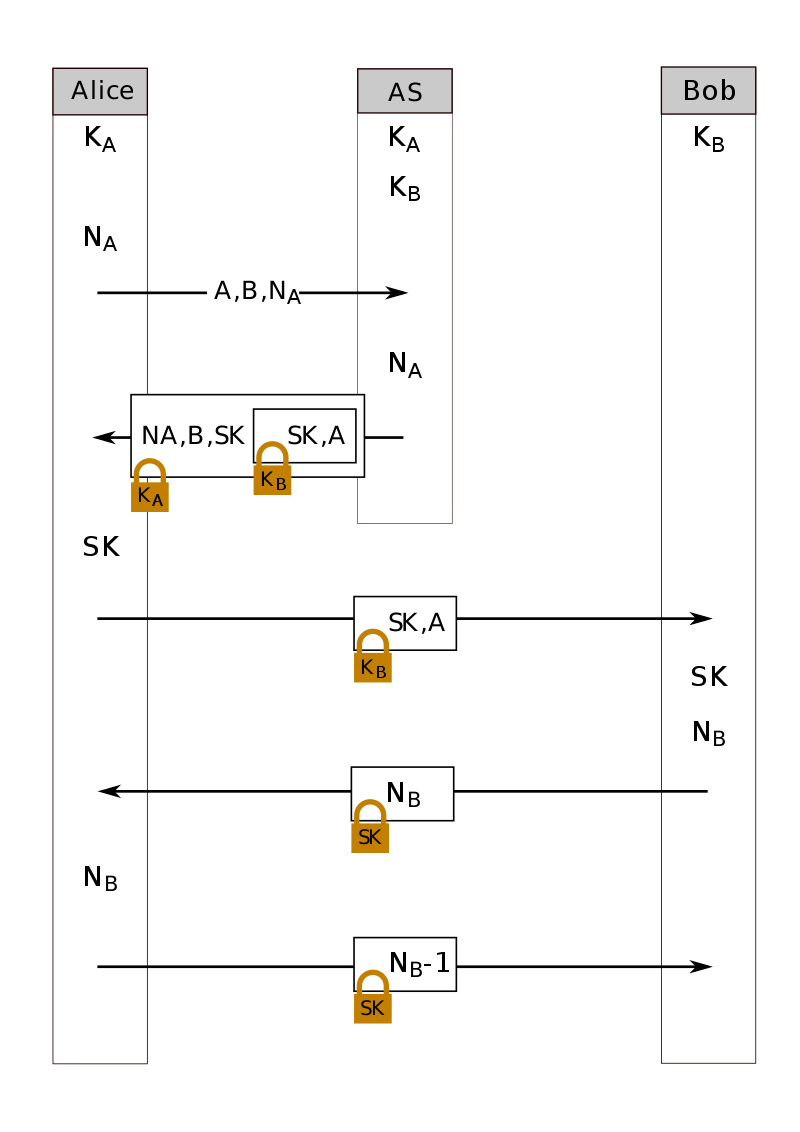
\includegraphics[scale=0.35]{ns.png}
\end{figure}
\begin{figure} [H]
    \centering
    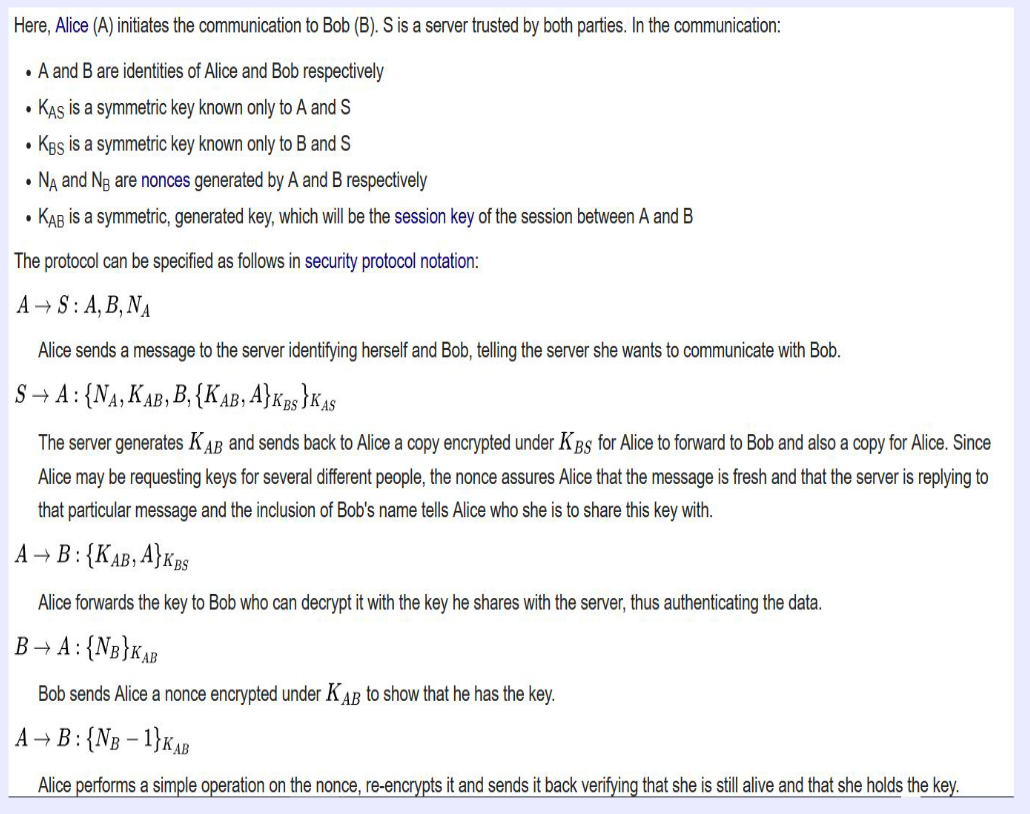
\includegraphics[scale=0.4]{ns_explain.png}
    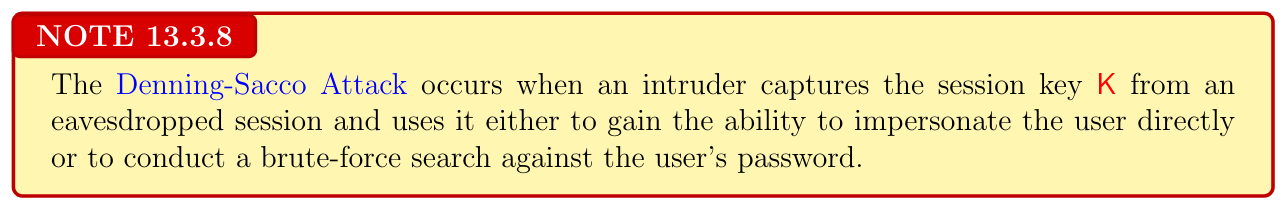
\includegraphics[scale=0.3]{denning.png}
\end{figure}
\end{document}

